\documentclass[11pt,a4paper]{article}

\usepackage[margin=1in]{geometry}
\usepackage[T1]{fontenc}
\usepackage[utf8]{inputenc}
\usepackage{lmodern}
\usepackage{microtype}
\usepackage{setspace}
\usepackage{booktabs}
\usepackage{tabularx}
\usepackage{longtable}
\usepackage{enumitem}
\usepackage{hyperref}
\usepackage{amsmath}
\usepackage{graphicx}
\usepackage{float}
\usepackage{tikz}
\usetikzlibrary{positioning,arrows.meta,shapes.geometric}

\hypersetup{
  colorlinks=true,
  linkcolor=blue!60!black,
  urlcolor=blue!60!black,
  citecolor=blue!60!black,
  pdftitle={Final Report: Fake News and Misinformation Detection System},
  pdfauthor={Seminar Project Team}
}

\setstretch{1.2}
\setlength{\parindent}{0pt}
\setlength{\parskip}{0.45em}
\renewcommand{\arraystretch}{1.15}

\title{Fake News \& Misinformation Detection System\\\large Final Report}
\author{Seminar Project Team}
\date{\today}

\begin{document}

\maketitle
\tableofcontents
\newpage

\section{Business Problem Definition and Project Objective}
\subsection{Business Context and Motivation}
Misinformation can spread faster than manual fact-checking teams can respond. In real operations such as media moderation, newsroom verification, and community trust-and-safety, the main pain points are high review volume, short response time, and inconsistent decision quality across reviewers. This project addresses that operational gap with an NLP-driven decision-support system that performs first-pass triage and provides evidence-aware explanations.

\subsection{Target Users and Stakeholders}
The intended users are moderators, verification staff, and analysts who need quick but reviewable assessments of article-like claims. Stakeholders include platform operators and project supervisors who evaluate whether the system is accurate, explainable, and deployable with limited resources.

\subsection{Why NLP Is Required}
The input is unstructured natural language text. Detecting misinformation requires understanding semantics, context, negation, and claim framing, which are not reliably captured by rule-only approaches. Therefore, NLP models are needed for scalable and consistent text understanding.

\subsection{Success Metrics}
The project uses measurable success criteria in both business and technical dimensions.

\begin{table}[H]
\centering
\caption{Project success metrics}
\label{tab:success-metrics}
\begin{tabularx}{\textwidth}{lX}
\toprule
Metric Type & Metrics \\
\midrule
Business metrics & Faster first-pass review, reduced manual triage effort, improved prioritization for human verification \\
Technical metrics & Accuracy, precision, recall, F1-score, API latency, uncertainty/conflict rate in agent workflow \\
\bottomrule
\end{tabularx}
\end{table}

\section{Development Infrastructure and Software Engineering Practice}
The project follows production-oriented software development rather than notebook-only experimentation. The implementation is in Python, version-controlled with Git, and organized as modular packages.

\subsection{Repository Structure}
The repository includes the expected production-style structure:
\begin{itemize}[leftmargin=1.2em]
  \item \texttt{src/}: backend, agent workflow, model inference, data and monitoring modules.
  \item \texttt{data/}: data files and data scripts.
  \item \texttt{models/}: saved baseline and transformer artifacts.
  \item \texttt{configs/}: YAML-based configuration for model, data, training, monitoring, and retrieval.
  \item \texttt{tests/}: unit and API tests for workflow and endpoints.
\end{itemize}

\subsection{Dependency and Reproducibility Setup}
Dependencies are managed via \texttt{requirements.txt} and project metadata in \texttt{pyproject.toml}. The project includes Docker configuration for reproducible local deployment. The README documents environment setup, training, inference, and serving commands.

\section{Data Management}
\subsection{Data Source and Licensing Notes}
The pipeline is configured around a local FakeNewsNet-style CSV dataset with text and binary label columns. The project documents source assumptions and treats dataset licensing and provenance as part of responsible data handling.

\subsection{Dataset Characteristics}
The system is designed for English-language news-like text with labels \texttt{fake} and \texttt{real}. Dataset quality is evaluated through split consistency, class balance awareness, and post-training error inspection.

\subsection{Preprocessing and Cleaning}
Preprocessing includes HTML and URL removal, text normalization, duplicate filtering, and empty-text handling. These steps are implemented as reusable code modules to keep the pipeline deterministic and auditable.

\subsection{Train/Validation/Test Strategy}
Data is split into 70\% train, 15\% validation, and 15\% test with stratification and fixed random seed. This supports fair comparison between baseline and transformer models.

\subsection{Known Limitations and Bias Risks}
Potential risks include topic imbalance, source-domain bias, and limited generalization to out-of-domain claims. These limitations are acknowledged in evaluation, monitoring, and ethics sections rather than hidden.

\section{Model Selection and Optimization}
\subsection{Model Choice Justification}
Two model families are used:
\begin{itemize}[leftmargin=1.2em]
  \item Baseline: TF-IDF + Logistic Regression for interpretability and fast benchmarking.
  \item Main model: RoBERTa for contextual understanding and stronger semantic representation.
\end{itemize}

This combination satisfies both practical benchmarking and high-performance modeling requirements.

\subsection{Training and Tuning Procedure}
The baseline is trained with sparse features and class-balanced logistic regression. The transformer is fine-tuned from \texttt{roberta-base} with tuned learning rate, sequence length, and checkpoint selection based on validation F1. Hyperparameter tuning is performed at least at a basic level through configured search choices.

\subsection{Baseline Comparison and Results}
\begin{table}[H]
\centering
\caption{Model evaluation summary}
\label{tab:model-results}
\begin{tabular}{lcccc}
\toprule
Model & Accuracy & Precision & Recall & F1 \\
\midrule
TF-IDF + Logistic Regression & 0.9913 & 0.9938 & 0.9870 & 0.9904 \\
RoBERTa & 0.9991 & 0.9987 & 0.9997 & 0.9992 \\
\bottomrule
\end{tabular}
\end{table}

As shown in Table~\ref{tab:model-results}, RoBERTa outperforms the baseline across all reported metrics.

\subsection{Error Analysis and Trade-offs}
Observed failure modes include ambiguous claims, weak-evidence scenarios, and noisy out-of-domain phrasing. In the latest live retrieval hardening pass, the system was improved with claim-centric queries, domain-aware fallback, and direct NASA source recovery for science claims; however, external search providers can still miss the intended authoritative page or return noisy concept pages before the fallback path activates. The key trade-offs are:
\begin{itemize}[leftmargin=1.2em]
  \item Accuracy vs speed: transformer is stronger but heavier than baseline.
  \item Complexity vs maintainability: agent-enabled pipeline is more useful but requires stronger integration testing and monitoring.
  \item Retrieval robustness vs dependency on external search providers: more aggressive fallback improves recall but increases integration complexity.
\end{itemize}

\section{Deployment Architecture and Inference Pipeline}
\subsection{Deployment Format}
The system provides both a REST API and a web-based demo:
\begin{itemize}[leftmargin=1.2em]
  \item FastAPI backend with endpoints \texttt{/predict}, \texttt{/analyze}, \texttt{/agent}, \texttt{/health}, and \texttt{/version}.
  \item Streamlit frontend for user interaction and result visualization.
\end{itemize}

\subsection{Input and Output Format}
Input is article text. Output includes predicted label, confidence, evidence summary, trust score, and explanation fields (depending on endpoint).

\subsection{Architecture Diagram}
Figure~\ref{fig:system-architecture} summarizes the deployed system.

\begin{figure}[H]
\centering
\makebox[\textwidth][c]{%
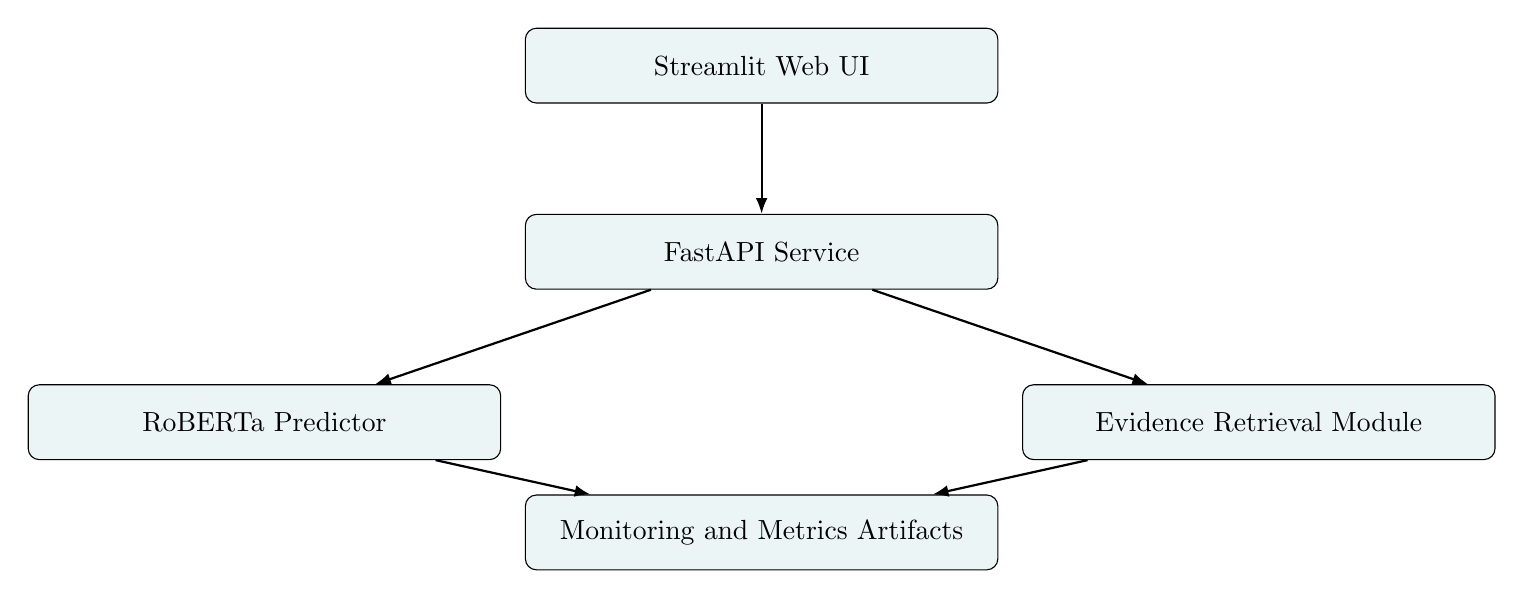
\begin{tikzpicture}[
  node distance=1.4cm,
  block/.style={draw, rounded corners, fill=teal!8, minimum width=6.0cm, minimum height=0.95cm, align=center},
  arrow/.style={-{Latex[length=2mm]}, thick}
]
\node[block] (ui) {Streamlit Web UI};
\node[block, below=of ui] (api) {FastAPI Service};
\node[block, below left=1.2cm and 0.3cm of api] (model) {RoBERTa Predictor};
\node[block, below right=1.2cm and 0.3cm of api] (retrieval) {Evidence Retrieval Module};
\node[block, below=2.6cm of api] (monitor) {Monitoring and Metrics Artifacts};
\draw[arrow] (ui) -- (api);
\draw[arrow] (api) -- (model);
\draw[arrow] (api) -- (retrieval);
\draw[arrow] (model) -- (monitor);
\draw[arrow] (retrieval) -- (monitor);
\end{tikzpicture}
}
\caption{Deployed architecture of the fake news detection system.}
\label{fig:system-architecture}
\end{figure}

\subsection{Deployment Constraints and Limitations}
Main constraints are free-tier resource limits, model size, and dependence on external evidence sources. These limitations are documented and reflected in risk management.

The live retrieval layer is intentionally conservative: when search quality is weak, the system may return \texttt{UNCERTAIN} rather than fabricate evidence. This is preferable for seminar evaluation, but it means some correct claims can still be misclassified or under-supported if the classifier is overconfident or the search provider is noisy.

\section{Agentic AI Component}
\subsection{Agent Architecture}
The project includes explicit multi-step agentic behavior through a controller that coordinates classifier, evidence retrieval, decision logic, and explanation generation.

\subsection{Flow and Decision Logic}
Figure~\ref{fig:agent-flow} shows the implemented sequence.

\begin{figure}[H]
\centering
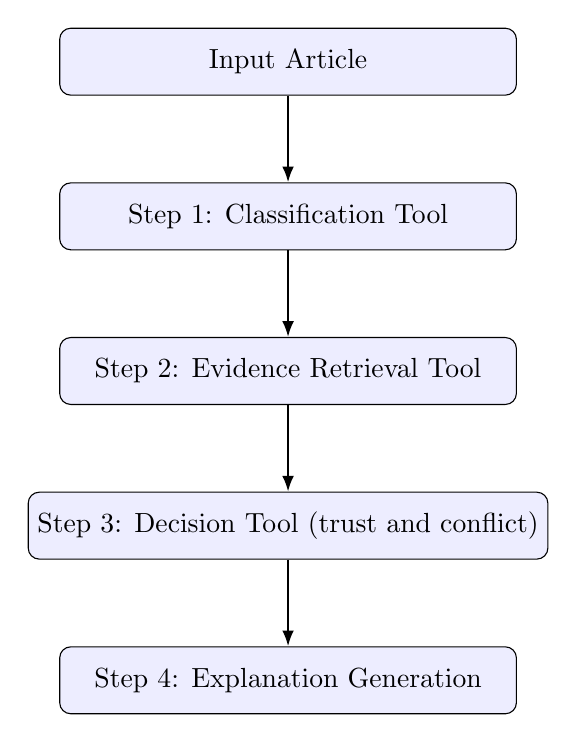
\begin{tikzpicture}[
  node distance=1.1cm,
  block/.style={draw, rounded corners, fill=blue!7, minimum width=5.8cm, minimum height=0.85cm, align=center},
  arrow/.style={-{Latex[length=2mm]}, thick}
]
\node[block] (input) {Input Article};
\node[block, below=of input] (classify) {Step 1: Classification Tool};
\node[block, below=of classify] (evidence) {Step 2: Evidence Retrieval Tool};
\node[block, below=of evidence] (decision) {Step 3: Decision Tool (trust and conflict)};
\node[block, below=of decision] (explain) {Step 4: Explanation Generation};
\draw[arrow] (input) -- (classify);
\draw[arrow] (classify) -- (evidence);
\draw[arrow] (evidence) -- (decision);
\draw[arrow] (decision) -- (explain);
\end{tikzpicture}
\caption{Agentic workflow with intermediate decision signals.}
\label{fig:agent-flow}
\end{figure}

\subsection{Example Interaction Behavior}
The agent can emit an \texttt{UNCERTAIN} review state when confidence is low or evidence conflicts with prediction. This demonstrates decision-making based on intermediate outputs, not single-pass labeling. Recent runtime traces also show why this matters: a science claim may now recover authoritative NASA evidence after fallback, while noisy claim wording can still initially attract irrelevant pages before the retrieval gate filters them out.

\section{Continual Learning and Monitoring Strategy}
The project includes a practical monitoring design and a conceptual continual-learning plan.

\subsection{Monitoring Metrics}
\begin{table}[H]
\centering
\caption{Monitoring metrics and purpose}
\label{tab:monitoring-metrics}
\begin{tabularx}{\textwidth}{lX}
\toprule
Metric & Purpose \\
\midrule
Confidence trend & Detect confidence degradation over time \\
Prediction distribution drift & Identify label skew changes \\
Data drift indicators & Detect input pattern shifts \\
Agent uncertain/conflict rate & Track reliability of evidence-assisted decisions \\
Latency and error rate & Monitor deployment stability \\
\bottomrule
\end{tabularx}
\end{table}

\subsection{Continual Learning Plan}
New data would be collected from reviewed uncertain/error cases, validated by human checks, and added to periodic retraining batches. Retraining would be triggered by threshold breaches in drift and uncertainty metrics.

\section{Data Privacy and Model Robustness}
\subsection{Privacy Handling}
The system masks personally identifiable information before inference and logging, reducing exposure of sensitive strings in artifacts and logs.

\subsection{Robustness Considerations}
The system explicitly addresses noisy and out-of-domain inputs by:
\begin{itemize}[leftmargin=1.2em]
  \item exposing uncertainty states,
  \item capturing evidence conflict,
  \item documenting failure cases for reviewer escalation.
\end{itemize}

\subsection{Mitigation Strategy}
Mitigations include conservative decision thresholds, human review escalation, and monitoring-driven retraining priorities.

\section{Project Management and Teamwork Reflection}
\subsection{Project Plan and Task Breakdown}
The project was executed in staged milestones: data and baseline setup, transformer training, agent integration, frontend/backend deployment, and final hardening.

\begin{table}[H]
\centering
\caption{Team-style task breakdown (solo simulation)}
\label{tab:team-breakdown}
\begin{tabularx}{\textwidth}{lX}
\toprule
Role Focus & Responsibilities \\
\midrule
ML engineer role & data preprocessing, baseline and transformer training, evaluation artifacts \\
Backend engineer role & API design, inference integration, endpoint validation, monitoring hooks \\
Frontend engineer role & Streamlit interaction flow, result visualization, user-facing error handling \\
MLOps/release role & deployment scripts, Docker setup, reproducibility and final submission packaging \\
\bottomrule
\end{tabularx}
\end{table}

\subsection{Scale-up Reflection}
In a real team, this project would scale with clearer service ownership, CI/CD checks per component, and shared monitoring dashboards.

\section{Ethics and Responsible AI}
\subsection{Who Benefits and Who May Be Harmed}
Benefits include faster reviewer triage and more structured claim analysis. Potential harms include false positives impacting legitimate content and false negatives allowing misinformation to pass.

\subsection{Bias and Fairness Risks}
Bias can arise from dataset composition, source imbalance, and domain mismatch. The project mitigates this through explicit limitation reporting, error analysis, and cautious interpretation of model outputs.

\subsection{Explainability for Non-technical Stakeholders}
The UI presents prediction, trust, evidence summary, and uncertainty state in plain language to support human decision-making.

\subsection{Potential Misuse}
Possible misuse includes over-reliance on automated outputs without human verification. The project mitigates this by surfacing uncertainty and recommending human review for ambiguous cases.

\section{Conclusion}
This project satisfies the assignment requirements by delivering an end-to-end, production-minded NLP system with clear business framing, structured data management, baseline and transformer comparison, agentic reasoning, deployable interfaces, monitoring strategy, privacy handling, and ethical reflection.

The main technical achievement is not only high classification performance but also integration of evidence-aware decision logic and explainability to support trustworthy operation.

\begin{thebibliography}{9}
\bibitem{devlin2019bert}
Devlin, J., Chang, M.-W., Lee, K., and Toutanova, K. (2019). BERT: Pre-training of Deep Bidirectional Transformers for Language Understanding.

\bibitem{liu2019roberta}
Liu, Y., Ott, M., Goyal, N., et al. (2019). RoBERTa: A Robustly Optimized BERT Pretraining Approach.

\bibitem{fakenewsnet}
Shu, K., Mahudeswaran, D., and Liu, H. (2018). FakeNewsNet: A Data Repository with News Content, Social Context and Dynamic Information.

\bibitem{fastapi}
FastAPI documentation. \url{https://fastapi.tiangolo.com/}

\bibitem{streamlit}
Streamlit documentation. \url{https://streamlit.io/}
\end{thebibliography}

\end{document}
